

%%%%%%%%%%%%%%%%%%%%%%%%%%%%%%%%%%% Introduction to ViennaCL %%%%%%%%%%%%%%%%%%%%%%%%%%%%%%%%%%%%


\begin{frame}{ }
 \begin{center}
  \Large \textbf{Introduction to \ViennaCL}
 \end{center}
\end{frame}


\begin{frame}{Introduction to \ViennaCL}

\begin{block}{What to expect}
  \begin{itemize}
   \item What is ViennaCL
   \item OpenCL
   \item History of ViennaCL
   \item Goals of ViennaCL
   \item Installation of ViennaCL
  \end{itemize}
\end{block}

\end{frame}




\begin{frame}{What Is \ViennaCL?}

\begin{block}{What is it about the Name?}
\begin{itemize}
  \item The beautiful city of \textbf{Vienna}
  \item Open\textbf{CL}
\end{itemize}
\end{block}

\vspace{3.4cm}

\end{frame}


% \begin{frame}{What Is \ViennaCL?}
% 
% \begin{block}{What is it about the Name?}
% \begin{itemize}
%   \item The beautiful city of \textbf{Vienna}
%   \item Open\textbf{CL}
% \end{itemize}
% \end{block}
% 
% {
% \centering
% 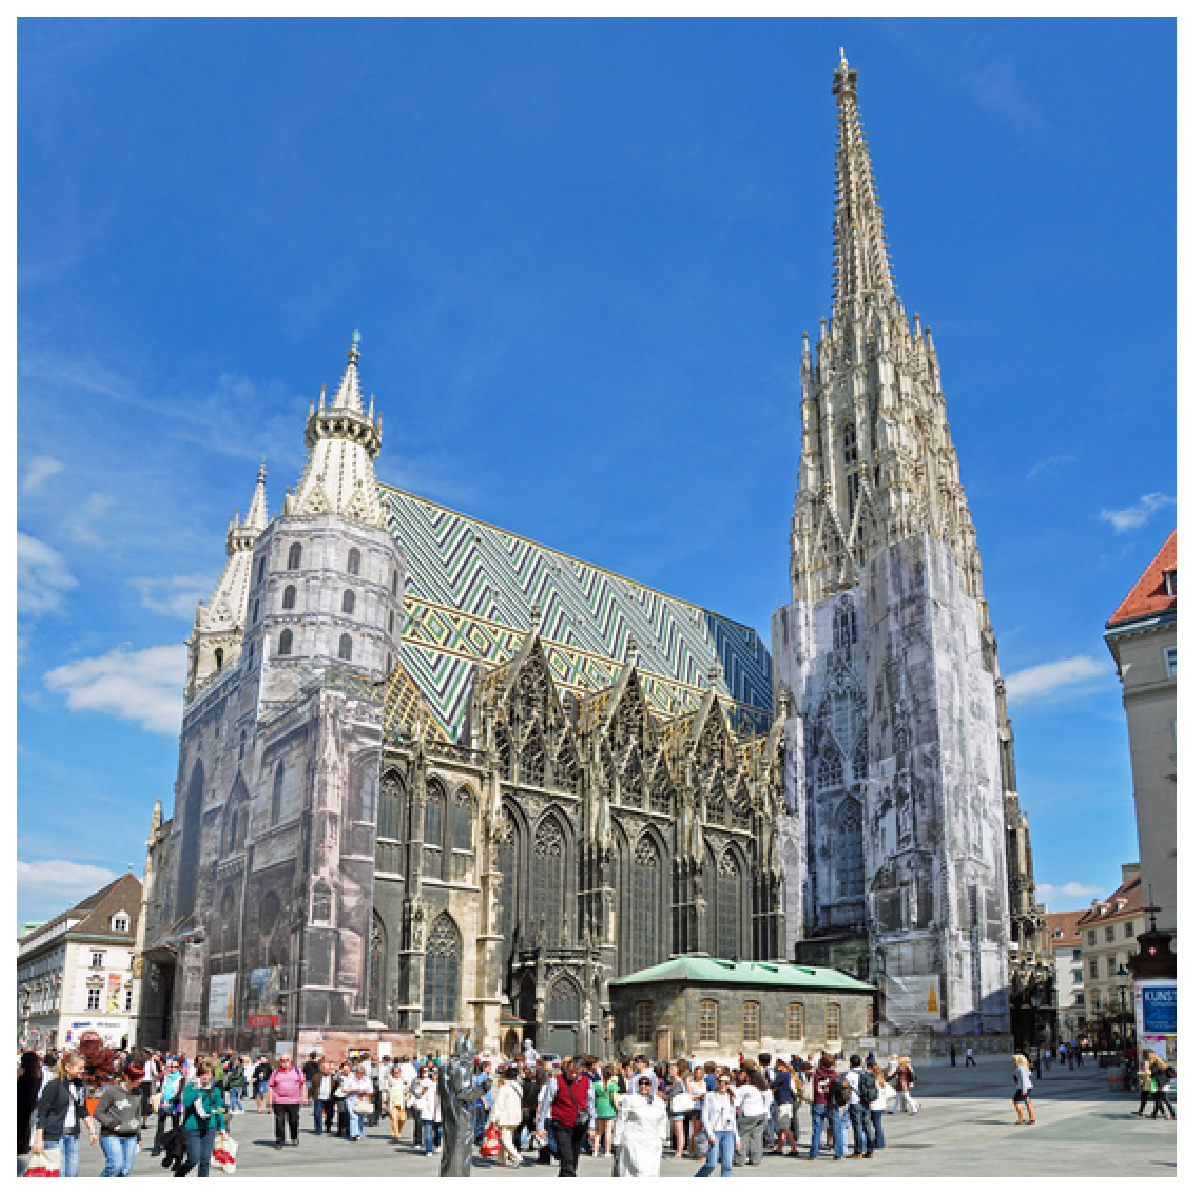
\includegraphics[width=0.3\textwidth]{figs/vienna.eps}
% }
% 
% \end{frame}


% \begin{frame}{What Is \ViennaCL?}
% 
% \begin{block}{What is it about the Name?}
% \begin{itemize}
%   \item The beautiful city of \textbf{Vienna}
%   \item Open\textbf{CL}
% \end{itemize}
% \end{block}
% 
% {
% \centering
% 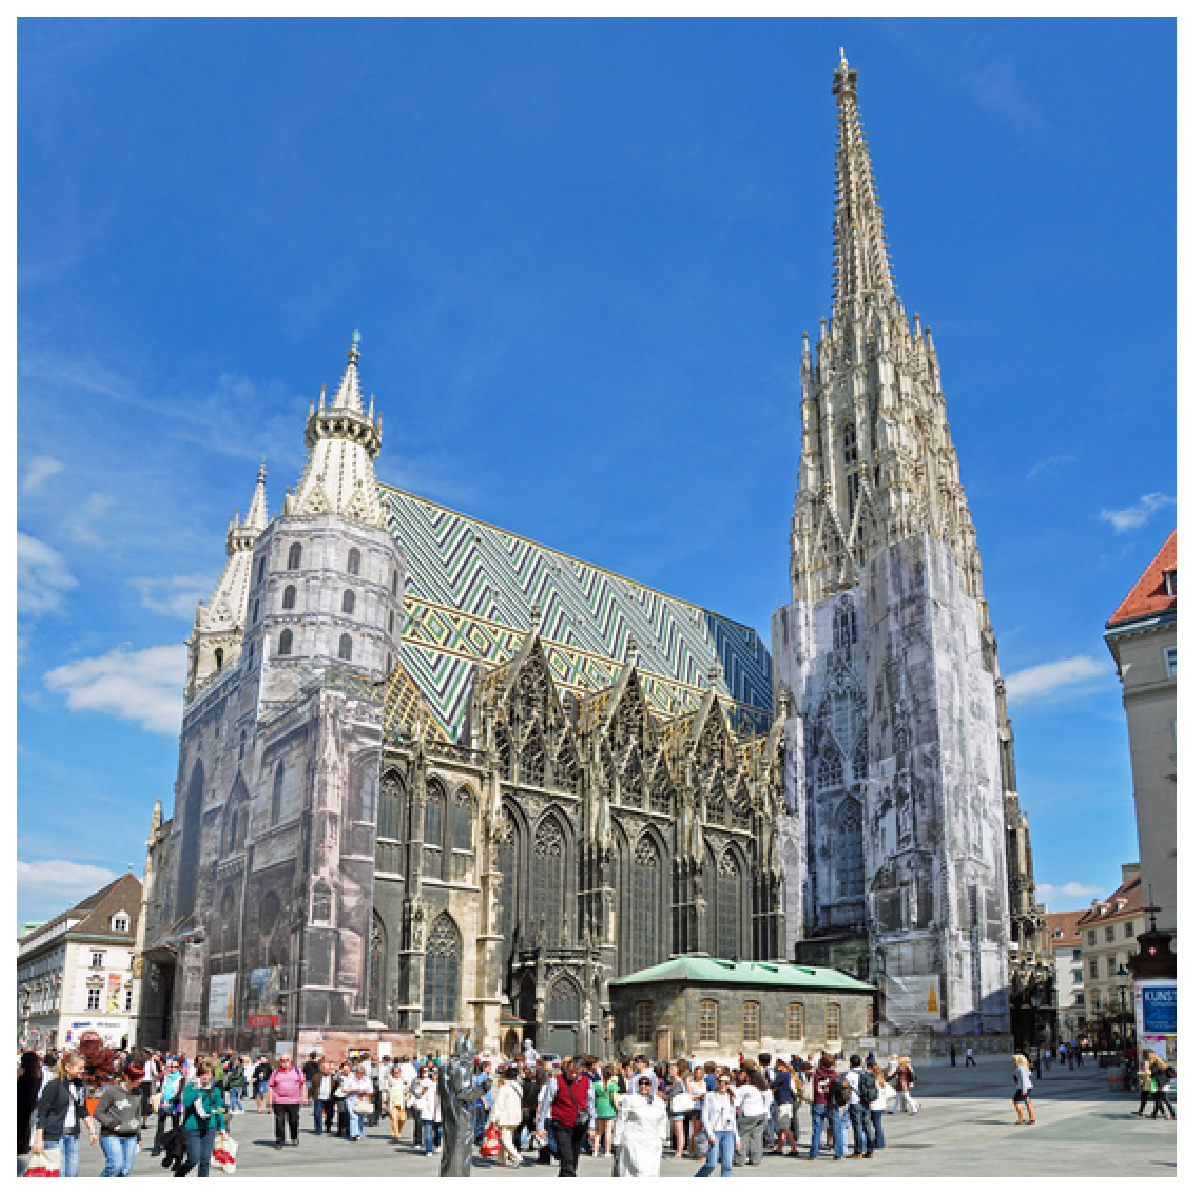
\includegraphics[width=0.3\textwidth]{figs/vienna.eps}
% \hspace{2cm}
% 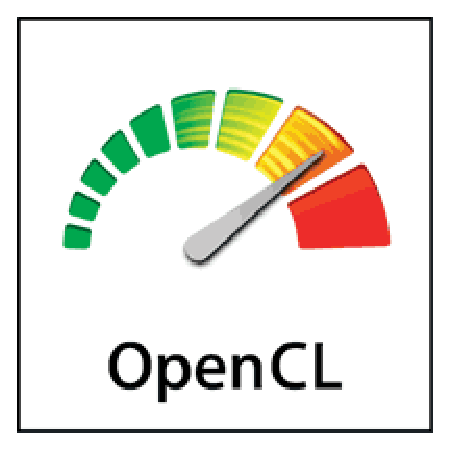
\includegraphics[width=0.3\textwidth]{figs/opencl_logo.eps}
% }
% 
% \end{frame}



\input{opencl}



\begin{frame}{History of \ViennaCL}

\begin{block}{2010}
  \begin{itemize}
   \item April: Roots in the Master's Thesis of Florian Rudolf
   \item May 28th: ViennaCL 1.0.0 released
   \item November: 1000th download
   \item December: ViennaCL 1.1.0 \\(BLAS level 3, refurbished OpenCL backend)
  \end{itemize}
\end{block}

\vspace*{2.49cm}
\end{frame}



\begin{frame}{History of \ViennaCL}

\begin{block}{2010}
  \begin{itemize}
   \item April: Roots in the Master's Thesis of Florian Rudolf
   \item May 28th: ViennaCL 1.0.0 released
   \item November: 1000th download
   \item December: ViennaCL 1.1.0 \\(BLAS level 3, refurbished OpenCL backend)
  \end{itemize}
\end{block}

\begin{block}{2011}
  \begin{itemize}
   \item March: Accepted for Google Summer of Code
   \item December: ViennaCL 1.2.0 \\ (AMG, SPAI, FFT, QR, graph algorithms, structured matrices)
  \end{itemize}
\end{block}

\end{frame}



\begin{frame}{History of \ViennaCL}

\begin{block}{2012}
  \begin{itemize}
   \item March: Accepted for Google Summer of Code
   \item May: Tutorial at NVIDIA GTC 2012
   \item May: ViennaCL 1.3.0 \\ (ranges and slices, Automated OpenCL kernels, eigen values, ILU0, SVD)
   \item December: ViennaCL 1.4.0 \\ (CUDA and host backend, initializer types)
  \end{itemize}
\end{block}

\vspace{2.07cm}

\end{frame}


\begin{frame}{History of \ViennaCL}

\begin{block}{2012}
  \begin{itemize}
   \item March: Accepted for Google Summer of Code
   \item May: Tutorial at NVIDIA GTC 2012
   \item May: ViennaCL 1.3.0 \\ (ranges and slices, Automated OpenCL kernels, eigen values, ILU0, SVD)
   \item December: ViennaCL 1.4.0 \\ (CUDA and host backend, initializer types)
  \end{itemize}
\end{block}

\begin{block}{2013}
  \begin{itemize}
   \item May: Accepted for Google Summer of Code
   \item June: Tutorial at CGLibs
  \end{itemize}
\end{block}

\end{frame}


% \begin{frame}{History of \ViennaCL}
% 
% \TODO{Achievement unlocked: Historian}
% 
% \end{frame}



\begin{frame}{Goals of \ViennaCL}

  \begin{block}{About}
   \begin{itemize}
    \item High-level linear algebra C++ library
    \item OpenMP, OpenCL, and CUDA backends
    \item Header-only
    \item Multi-platform
   \end{itemize}
  \end{block}

  \vspace*{-2.3cm}
  \begin{flushright}
   \includegraphics[width=0.4\textwidth]{figs/ViennaCL-arch.png}
  \end{flushright}

  \vspace*{-0.7cm}
  \begin{block}{Dissemination}
    \begin{itemize}
     \item Free Open-Source MIT (X11) License
     \item http://viennacl.sourceforge.net/
     \item 50-100 downloads per week
    \end{itemize}   
  \end{block}

  \begin{block}{Design Rules}
   \begin{itemize}
    \item Reasonable default values
    \item Compatible to Boost.uBLAS whenever possible 
    \item In doubt: clean design over performance
   \end{itemize}
  \end{block}

\end{frame}



\begin{frame}{Goals of \ViennaCL}

  \begin{block}{Core features}
    \begin{itemize}
     \item Linear algebra, BLAS
     \item Solver (direct and iterative)
     \item Preconditioners
    \end{itemize}   
  \end{block}
     
  \begin{block}{Additional features}
    \begin{itemize}
     \item Fast Fourier Transform
     \item Eigenvalue computations
     \item QR factorization
     \item Bandwidth reduction
     \item Nonnegative matrix factorization
    \end{itemize}   
  \end{block}

\end{frame}



\begin{frame}{Goals of \ViennaCL}

  \begin{block}{Interfaces to other libraries}
    \begin{itemize}
     \item Boost.uBLAS
     \item Eigen
     \item MTL4
    \end{itemize}   
  \end{block}

  \begin{block}{Backends}
   \begin{itemize}
    \item CPU
    \item OpenCL
    \item CUDA
   \end{itemize}
  \end{block}

  \begin{block}{C++ library}
   \begin{itemize}
    \item Generic free functions
    \item Expression templates
   \end{itemize}
  \end{block}

\end{frame}



\begin{frame}{Installation of \ViennaCL}

  \begin{block}{Three Steps}
    \begin{itemize}
     \item Download from http://viennacl.sourceforge.net/
     \item Unzip
     \item Copy source folder
    \end{itemize}   
  \end{block}

  \begin{block}{Dynamic Library?}
    \begin{itemize}
     \item ViennaCL is header-only
     \item Linking depends on used backend (OpenMP, OpenCL, CUDA)
    \end{itemize}
  \end{block}

  \begin{block}{Sample Applications}
    \begin{itemize}
     \item 22 tutorials
     \item $\hphantom{0}$7 benchmarks
     \item about 35 tests
    \end{itemize}
  \end{block}

\end{frame}

